\section{ML Testing Design}

% As part of the assignment on ML Testing, you had to design a testing strategy and implement
% some automated tests. In this section, we expect you to fully document your choices and to reflect on limitations
% of the existing testing strategy. Moreover, we would like to hear your thoughts on how to improve tests, which new
% tests should be implemented and why
This section will first describe and explain the tests implemented, it will then talk about the limitations and which additional tests could be added. Finally, it will explain what was done for continuous training.

\subsection{Automated Tests}
%DONT FORGET TO ADD WHY
%Divide into the big 4?
The tests created are there to ensure the functionality of the training pipeline, therefore they were implemented in the model-training repository.
\\\\
Here's a list of the different tests that were done:
\begin{itemize}
    \item Data quality tests: These tests are here to ensure the quality of the data, this is done by verifying the uniqueness of data samples, the data should at least be 99\% unique.
    \item Integration tests: These tests ensure that the complete pipeline can be run together without causing any issues, they follow the following pattern: preprocess the data, build the model, train the model, test the model, and plot
    \item Model definition test: Verify that the model is defined properly
    \item Model development tests:
    \begin{itemize}
        \item Capability test: Ensure that if the data (URL) starts with HTTP or HTTPS it yields similar results.
        \item Non-determinism test: Ensure that the training phase is nondeterministic and that the difference accuracy between 2 trained models should be minimal
    \end{itemize}

    \item Test monitoring: Ensure that it doesn't use too much RAM <4GB
    \item Test train: Ensure that the training phase returns a trained model
    \item Test Preprocess: Ensure data exists and that it has the right shape 
\end{itemize}

To improve the testing multiple things can be done, first, add more unit tests to increase the test coverage. Currently, none of the tests are using the DVC data, therefore it would be useful to add some. Finally, some metamorphic tests could be added.
\subsection{Continuous training}

To ensure the quality of our code, a testing pipeline was set up using GitHub workflows.

This pipeline will run the tests in each OS (Windows, MacOS, Linux) to ensure no dependency issues. Then, it will upload the results to Codecov as seen in Figure \ref{fig:codecov}.

\begin{figure}[h!]
    \centering
    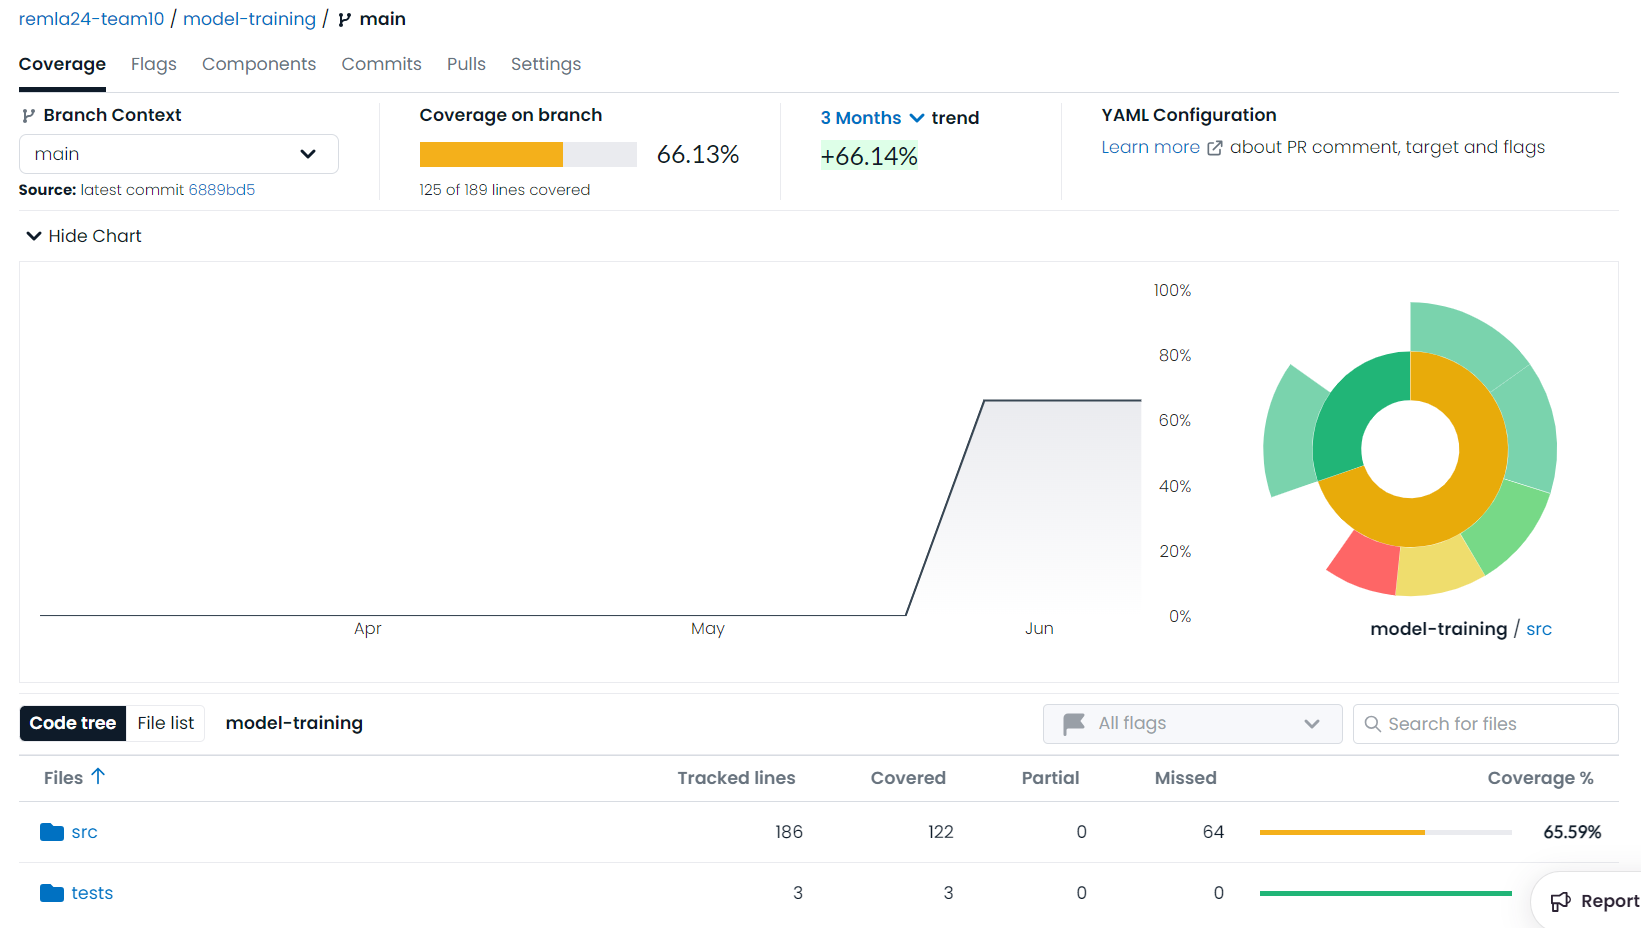
\includegraphics[width=0.5\textwidth]{images/codecov.png}
    \caption{Screenshot of Codecov dashboard of model-training}
    \label{fig:codecov}
\end{figure}

Then a test report will be created as shown in Figure \ref{fig:test_results}, it will show up as a comment in each merge request.

\begin{figure}[h!]
    \centering
    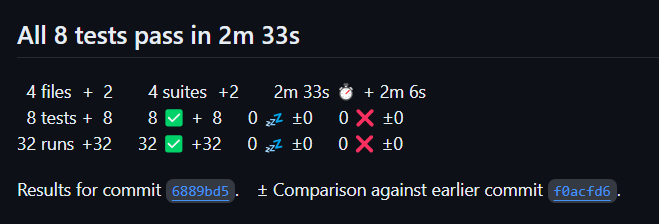
\includegraphics[width=0.3\textwidth]{images/test_results.png}
    \caption{Screenshot of a test report from the workflow}
    \label{fig:test_results}
\end{figure}

Finally, a badge is displayed as shown in Figure \ref{fig:badge} on the README with the results, this badge is updated every time we merge to the main branch.



\begin{figure}[h!]
    \centering
    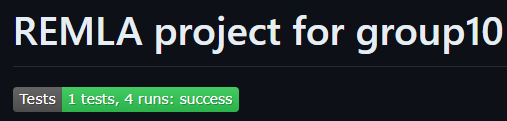
\includegraphics[width=0.3\textwidth]{images/test_badge.png}
    \caption{Screenshot of the badge}
    \label{fig:badge}
\end{figure}